\documentclass[conference]{IEEEtran}
\usepackage{amsmath,amssymb}
\usepackage{booktabs}
\usepackage{graphicx}
\usepackage{tikz}
\usetikzlibrary{arrows.meta,positioning}
\usepackage{url}
\usepackage{cite}
\title{Reproducibility Assessment of CRNN and GluNet for Personalized Blood Glucose Forecasting on OhioT1DM}
\author{\IEEEauthorblockN{Sulabh Yadav}\IEEEauthorblockA{Working manuscript; affiliations and target venue to be added}}
\begin{document}
\maketitle
\begin{abstract}
Continuous glucose monitoring (CGM) forecasting can support anticipatory diabetes management, but reported performance depends on cohort, preprocessing, prediction horizon, and evaluation protocol. This working manuscript documents a reproducibility study of a convolutional recurrent neural network (CRNN) and GluNet-style gated causal convolutions on the predefined OhioT1DM partitions. The repository contains preliminary 30- and 60-minute results, gap-aware sequence construction, patient-specific training code, and clinical metric utilities. The current implementations have not yet been established as exact reproductions of the source papers: the CRNN's Gaussian-filtering and modified-LSTM details remain unresolved, while the existing GluNet regression results use a continuous objective rather than the original 256-class formulation. Final comparative claims are withheld until paper-specific preprocessing, class decoding, clinical metrics, and extended horizons have been validated. Results will be populated from traceable run artifacts only.
\end{abstract}
\begin{IEEEkeywords}
continuous glucose monitoring, glucose forecasting, CRNN, GluNet, OhioT1DM, reproducibility, clinical evaluation
\end{IEEEkeywords}

\section{Introduction}
CGM forecasting is a time-series prediction problem with clinical implications. Short forecast horizons can support timely awareness of glucose changes, while evaluation must account for temporal autocorrelation, gaps in sensor data, patient heterogeneity, and the clinical consequences of prediction errors. This work focuses on reproducing two published architectures before proposing further hybrid-model changes.

\section{Related Work}
Li et al. introduced GluNet as a deep-learning framework for glucose forecasting using a discretized glucose-change prediction formulation \cite{li_glunet}. Li et al. also described a convolutional recurrent neural network with a modified recurrent output connection for glucose prediction \cite{li_crnn}. Results reported in those papers are literature results, not directly interchangeable with OhioT1DM results produced under different partitions, cohort sizes, or preprocessing.

\section{Materials and Methods}
\subsection{Dataset and partitions}
The study uses predefined OhioT1DM training and testing partitions for up to 12 subjects: 559, 563, 570, 575, 588, 591, 540, 544, 552, 567, 584, and 596. Raw XML data are governed by a data-use agreement and are not distributed in this repository. The training partition is divided chronologically into fitting and validation portions. The predefined test partition is reserved for final evaluation.

\subsection{Temporal alignment and gaps}
Inputs are aligned to the 5-minute CGM timeline. Windows and forecast targets must lie within one continuous segment, and target timestamps must match the requested horizon exactly. The current candidate pipeline splits at timestamp gaps rather than reproducing every source-paper interpolation rule. This is a documented adaptation until the original procedures are verified. Any future interpolation must record an eligibility mask so ineligible targets are not scored.

\subsection{Features}
The common primary feature set is CGM glucose, carbohydrate intake, and insulin bolus. Basal insulin and time-of-day encodings are treated as explicit adaptations when used. The physiological estimates $P_i$ and $R_a$ are optional extensions and are not included in the primary result until their equations, parameter assumptions, and implementation are validated.

\section{GluNet and CRNN Architectures}
\subsection{GluNet}
The candidate implementation uses a 16-step input and a 256-class glucose-change output. A class label is mapped to a quantized change and combined with current glucose to recover the forecast. The precise class-boundary convention and probability-to-point decoder must be tested against the source method before this candidate is called a faithful reproduction.

\subsection{CRNN}
The current candidate uses 24 input steps, three convolution/max-pooling stages, and a modified LSTM with a 64-unit hidden state. The implementation uses a learned projection when the convolutional output dimension differs from the recurrent hidden dimension. This is an adaptation; the published parameter-count discrepancy and exact Gaussian filtering configuration remain open items.

\begin{figure}[t]
\centering
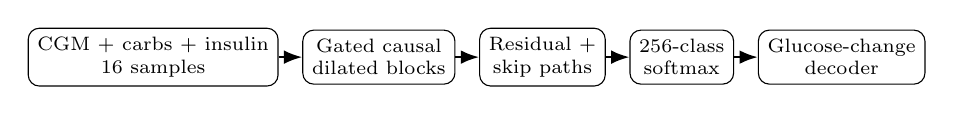
\begin{tikzpicture}[node distance=3mm, every node/.style={draw, rounded corners, align=center, font=\scriptsize, minimum height=6mm}, arr/.style={-{Latex},thick}]
\node (in) {CGM + carbs + insulin\\16 samples};
\node[right=of in] (causal) {Gated causal\\dilated blocks};
\node[right=of causal] (skip) {Residual +\\skip paths};
\node[right=of skip] (class) {256-class\\softmax};
\node[right=of class] (out) {Glucose-change\\decoder};
\draw[arr] (in)--(causal); \draw[arr] (causal)--(skip); \draw[arr] (skip)--(class); \draw[arr] (class)--(out);
\end{tikzpicture}
\caption{Schematic of the GluNet candidate. The final paper-aligned channel and layer configuration must be verified.}
\label{fig:glunet}
\end{figure}

\begin{figure}[t]
\centering
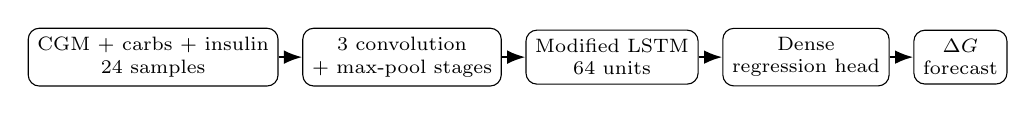
\begin{tikzpicture}[node distance=3mm, every node/.style={draw, rounded corners, align=center, font=\scriptsize, minimum height=6mm}, arr/.style={-{Latex},thick}]
\node (in) {CGM + carbs + insulin\\24 samples};
\node[right=of in] (conv) {3 convolution\\+ max-pool stages};
\node[right=of conv] (lstm) {Modified LSTM\\64 units};
\node[right=of lstm] (dense) {Dense\\regression head};
\node[right=of dense] (out) {$\Delta G$\\forecast};
\draw[arr] (in)--(conv); \draw[arr] (conv)--(lstm); \draw[arr] (lstm)--(dense); \draw[arr] (dense)--(out);
\end{tikzpicture}
\caption{Schematic of the current CRNN candidate; filtering and residual details remain subject to source-paper verification.}
\label{fig:crnn}
\end{figure}

\section{Experimental Setup and Evaluation Metrics}
The initial horizons are 30 and 60 minutes, followed by 15, 90, and 120 minutes. Training is patient-specific and uses fixed random seeds. Validation data are drawn chronologically from the training partition. The test set is not used for model selection.

We report root mean squared error (RMSE), mean absolute error (MAE), mean absolute relative difference (MARD), time lag, and Clarke Error Grid Analysis (zones A--E). Metrics are calculated patient-wise and summarized as the mean and sample standard deviation across patients. Time lag is computed within contiguous timestamp segments. Metric implementations require synthetic unit tests and an audit of final prediction tables before publication.

\section{Results and Discussion}
\subsection{Existing preliminary CRNN results}
The current repository audit reported the following preliminary 30- and 60-minute values. They are results of the current implementation, not proof of exact reproduction.

\begin{table}[t]
\centering
\caption{Preliminary CRNN results across patients (mean $\pm$ sample SD).}
\label{tab:crnn-preliminary}
\begin{tabular}{lrr}
\toprule
Metric & 30 min & 60 min \\
\midrule
MAE (mg/dL) & 13.494 $\pm$ 1.480 & 23.637 $\pm$ 2.714 \\
RMSE (mg/dL) & 19.309 $\pm$ 2.203 & 32.577 $\pm$ 3.718 \\
MARD (\%) & 9.073 $\pm$ 1.591 & 15.783 $\pm$ 2.755 \\
\bottomrule
\end{tabular}
\end{table}

\subsection{Existing GluNet-inspired regression results}
A separate existing experiment uses continuous Huber regression, not the original GluNet 256-class loss. It is reported here only as a project baseline.

\begin{table}[t]
\centering
\caption{Preliminary GluNet-inspired Huber-regression results (mean $\pm$ sample SD).}
\label{tab:glunet-regression}
\begin{tabular}{lrr}
\toprule
Metric & 30 min & 60 min \\
\midrule
MAE (mg/dL) & 13.526 $\pm$ 1.628 & 23.507 $\pm$ 3.419 \\
RMSE (mg/dL) & 19.318 $\pm$ 2.501 & 32.356 $\pm$ 4.375 \\
MARD (\%) & 9.114 $\pm$ 1.745 & 15.907 $\pm$ 3.342 \\
Time lag (min) & 21.528 $\pm$ 3.922 & 46.111 $\pm$ 9.753 \\
\bottomrule
\end{tabular}
\end{table}

These tables are not a head-to-head comparison: they reflect distinct implementations and metric coverage. Paper-faithful classifier results and complete CRNN clinical evaluation remain to be completed. The final version must include patient-wise tables and common-target-timestamp comparisons against existing GRU, LSTM, TCN, Transformer, hybrid, and persistence baselines.

\section{Statistical and Clinical Evaluation}
Patient is the unit of aggregation for mean and standard deviation; overlapping forecast windows are not treated as independent subjects. Paired comparisons will be performed only after predictions are aligned on identical target timestamps. Multiple-comparison adjustment and effect sizes will be reported for exploratory contrasts. Clarke Error Grid implementations will be checked against reference cases and independently reviewed before clinical claims.

\section{Limitations}
The cohort is small and limited to OhioT1DM. Existing implementations still have unresolved fidelity questions. The current candidate GluNet pipeline has not established exact source-paper class decoding or preprocessing. The CRNN Gaussian filtering and modified-LSTM parameterization remain unresolved. No external cohort validation or clinical deployment assessment is claimed.

\section{Conclusion and Future Work}
The repository provides a starting point for a reproducible benchmark, including preliminary results and gap-aware sequence construction. Next steps are to validate source-paper specifications, run the 30/60-minute experiments with isolated outputs, extend to 15/90/120 minutes, complete clinical metric validation, align predictions with existing baselines, and populate the manuscript from traceable experiment artifacts. A hybrid architecture should be developed only after these benchmarks are stable.

\bibliographystyle{IEEEtran}
\bibliography{ieee_reproduction_references}
\end{document}
